\documentclass{article}
\usepackage[utf8]{inputenc}
\usepackage{cite}
\usepackage{amsmath,amssymb,amsfonts}
\usepackage{graphicx}
\usepackage{textcomp}
\usepackage{xcolor}
\usepackage{booktabs}
\usepackage{multirow}
\usepackage{diagbox}
\usepackage{listings}
\usepackage{geometry}
\usepackage{verbatim}
\usepackage{subfigure}
\usepackage{abstract}
\usepackage{fancyhdr}
\usepackage{color}
\usepackage{float}
\usepackage{url}
\usepackage[colorlinks,linkcolor=blue,anchorcolor=blue,citecolor=red]{hyperref}
\usepackage{makecell}
\usepackage{indentfirst}
\usepackage{xcolor}
\lstset{
     %行号
     numbers=left,
     %背景框
     framexleftmargin=10mm,
     frame=none,
     %背景色
     %backgroundcolor=\color[rgb]{1,1,0.76},
     backgroundcolor=\color[RGB]{245,245,244},
     %样式
     keywordstyle=\bf\color{blue},
     identifierstyle=\bf,
     numberstyle=\color[RGB]{0,192,192},
     commentstyle=\it\color[RGB]{0,96,96},
     stringstyle=\rmfamily\slshape\color[RGB]{128,0,0},
     %显示空格
     showstringspaces=false
}
\setlength{\parindent}{2em}

\title{\textbf{Android Start Up\\Mobile Internet Lab1}}


\begin{document}
	\maketitle
	
	\begin{abstract}
		Learning basic knowledge of Java and Android programming. Realize Hello World and drawLine Program with my own design.
		
		\textit{\textbf{Key Words:} }Android Programming, Java, DrawLine
	\end{abstract}
	
	
	\section{Environment}
	I use Android Studio 3.6.2 with Oracle Java 1.8.0.
	
	\section{Project: Hello World}
	Hello World is my first java program. I realize it and change its binding string.
	
	To achieve the binding operation, I do with the following steps:
	\begin{enumerate}
		\item[*] Fine the TextView by id.
		\begin{lstlisting}[language={java}]
TextView txtResult = (TextView) findViewById(R.id.txtResult);
		\end{lstlisting}
		
		\item[*] And then give the TextView value.
		\begin{lstlisting}[language={java}]
txtResult.setText(String.valueOf(text));
		\end{lstlisting}
		
	\end{enumerate}

	\textbf{Demo}
	
	By moving these three TextView to different position, I have the folloing screenshooting.
	
	\begin{center}
	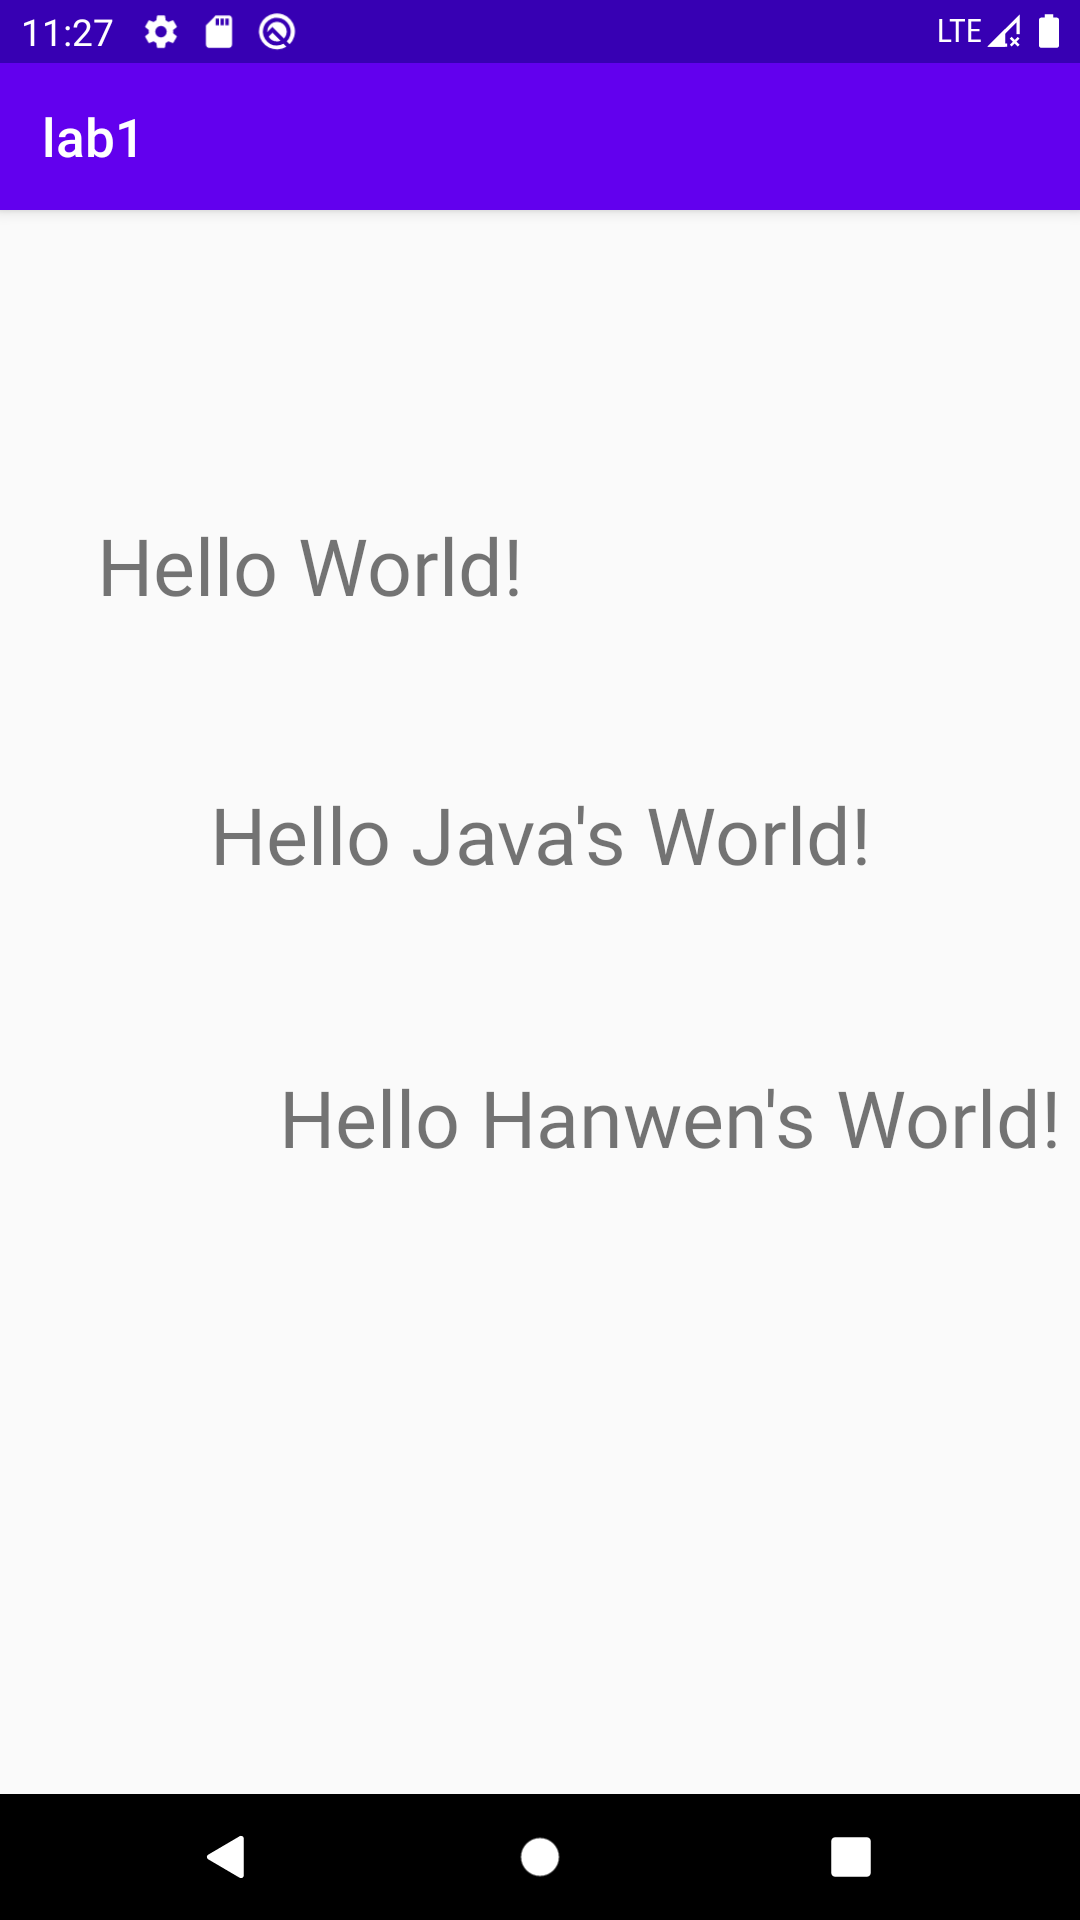
\includegraphics[scale=0.4]{demo.png}
	\end{center}
	
	\section{Project: DrawLine}
	
	This project realize a drawline application using finger touch. From Computer simulator, it follows the action detected from the mouse.
	
	What creativity I add in this program is automatically changing color, as the following two demos.
	
	\begin{center}
		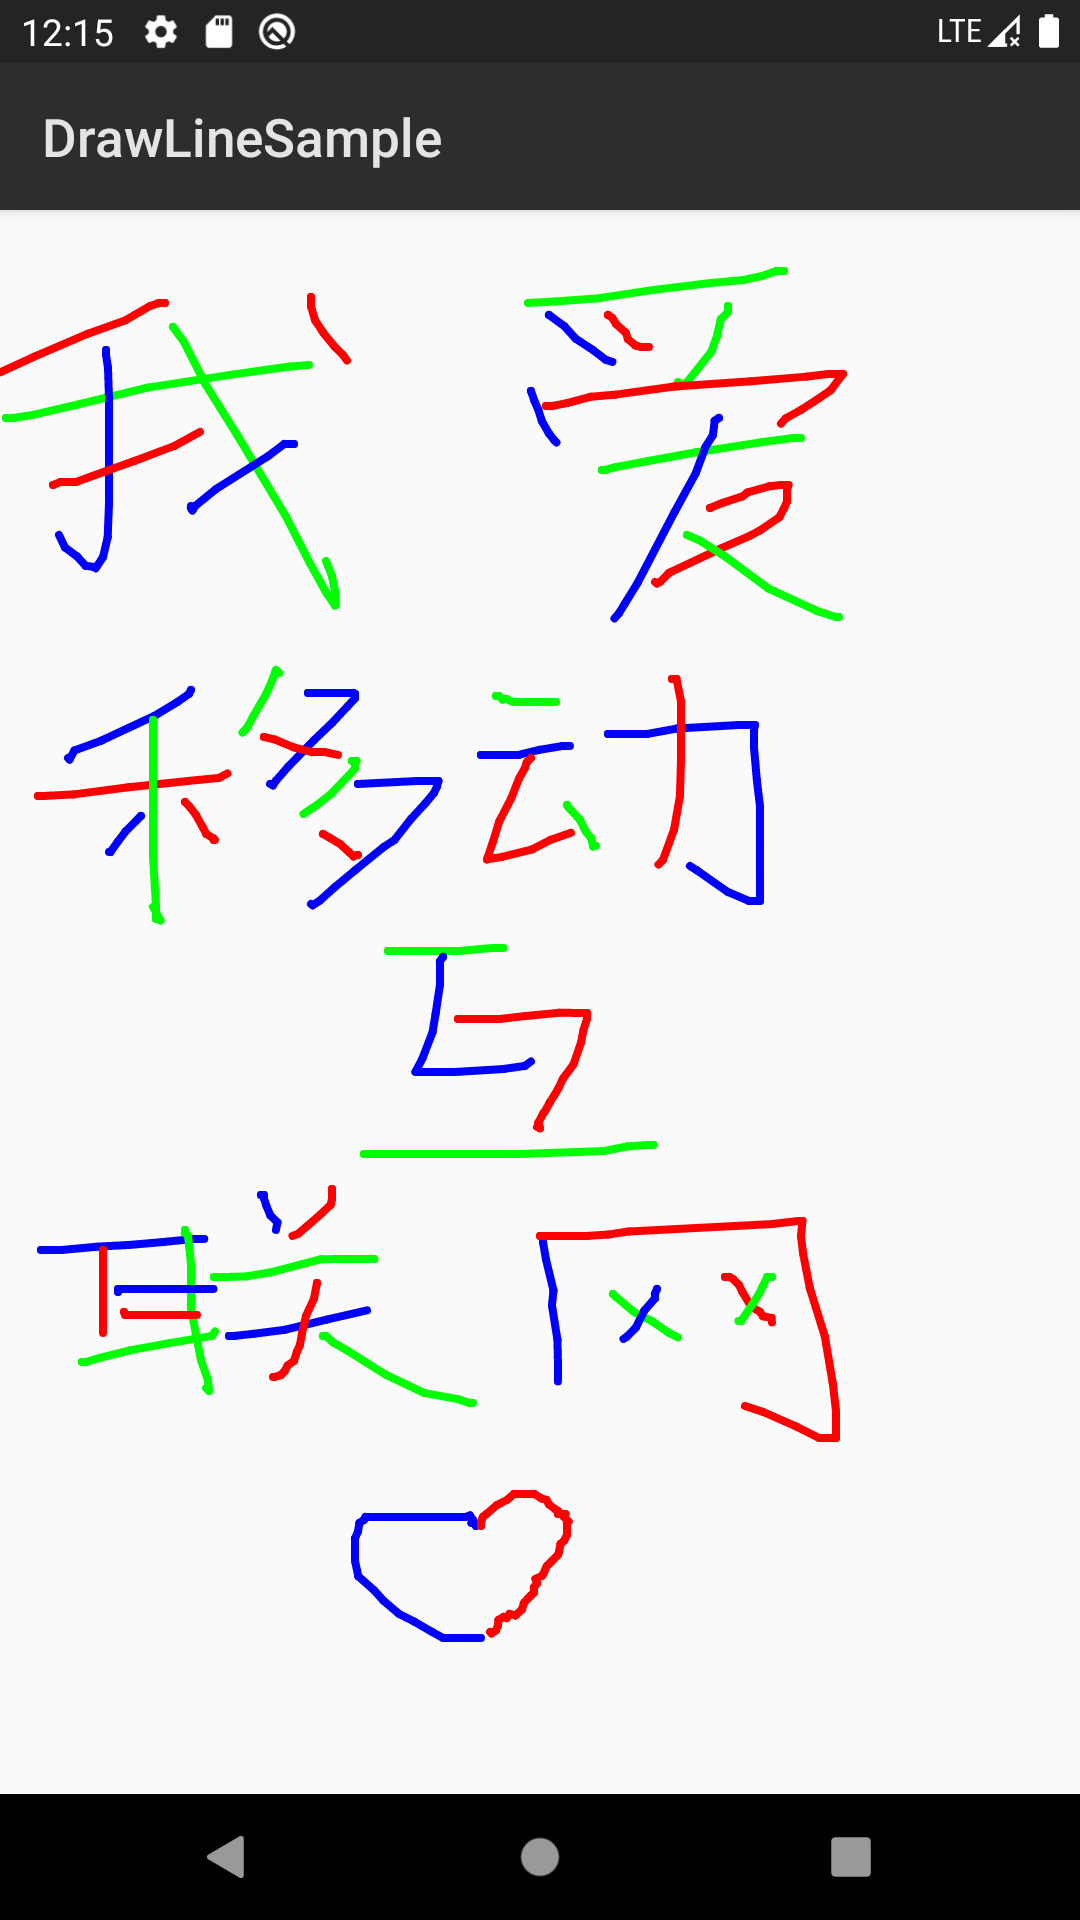
\includegraphics[scale=0.17]{love.png}
		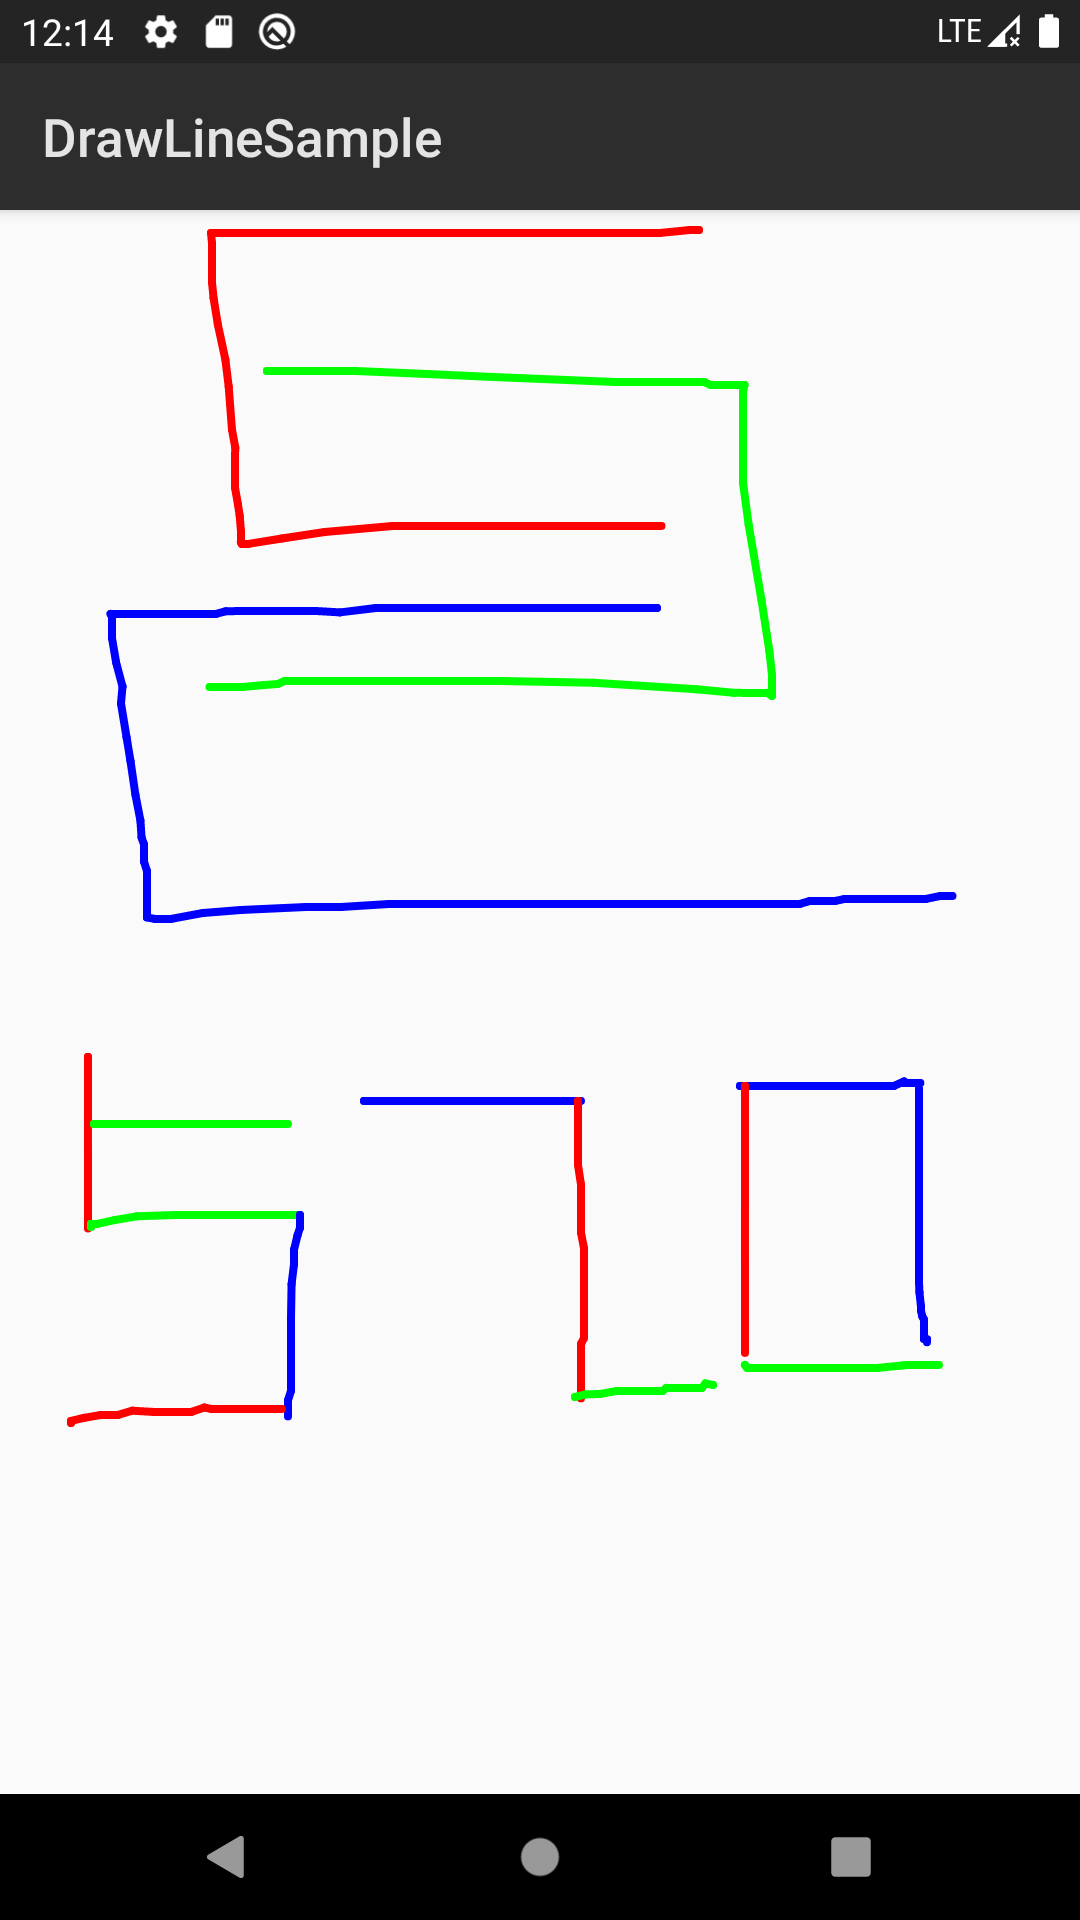
\includegraphics[scale=0.17]{Colorful_520.png}
	\end{center}

	I add switch method in Java in the ACTION\_UP function to realize changing the color. 
	
	\begin{lstlisting}[language={java}]
switch (time) {
case 0:
p.setColor(Color.GREEN);
break;
case 1:
p.setColor(Color.BLUE);
break;
case 2:
p.setColor(Color.RED);
break;
}
time = (time + 1) % 3;
	\end{lstlisting}
	
	In this process, I find some similarity between Java and C++. 
	
	And I also think, my program will be more interesting with random color choosing. While the code is easy to write and understand, I will not show it in the report.
	
	\section{Conclusion}
	The first Java lab introduces me into the Android World, I think it is very interesting to program with Java. I also update all my code and demo to my Github: https://github.com/david990917/My-Computer-Science-Learning/tree/master/Courses/Mobile-Internet/Lab1
	
	
	
	
\end{document}